\subsection{Definition}
\begin{frame}
  \frametitle{Definition}

  \begin{block}{Zweck}
  	Definition einer 1-zu-n-Abhängigkeit zwischen Objekten, damit im Fall einer Zustandsänderung eines Objekts alle davon abhängigen Objekte entsprechend benachrichtigt und automatisch aktualisiert werden.
  \end{block}
  
\end{frame}

\subsection{Klassendiagramm - Observer Pattern}

\begin{frame}
\frametitle{Klassendiagramm}
\begin{columns} 
    	\column[c]{.35\textwidth} 
    		\begin{itemize}
    			\item 1-zu-n-Abhänigkeit
    			\item Subject benachrichtig Observer
    			\item Zustandsänderung ist Auslöser
    			\item Clients aktualisieren sich selbst
    		\end{itemize}
    	\column[c]{.65\textwidth} 
    			\begin{figure}
					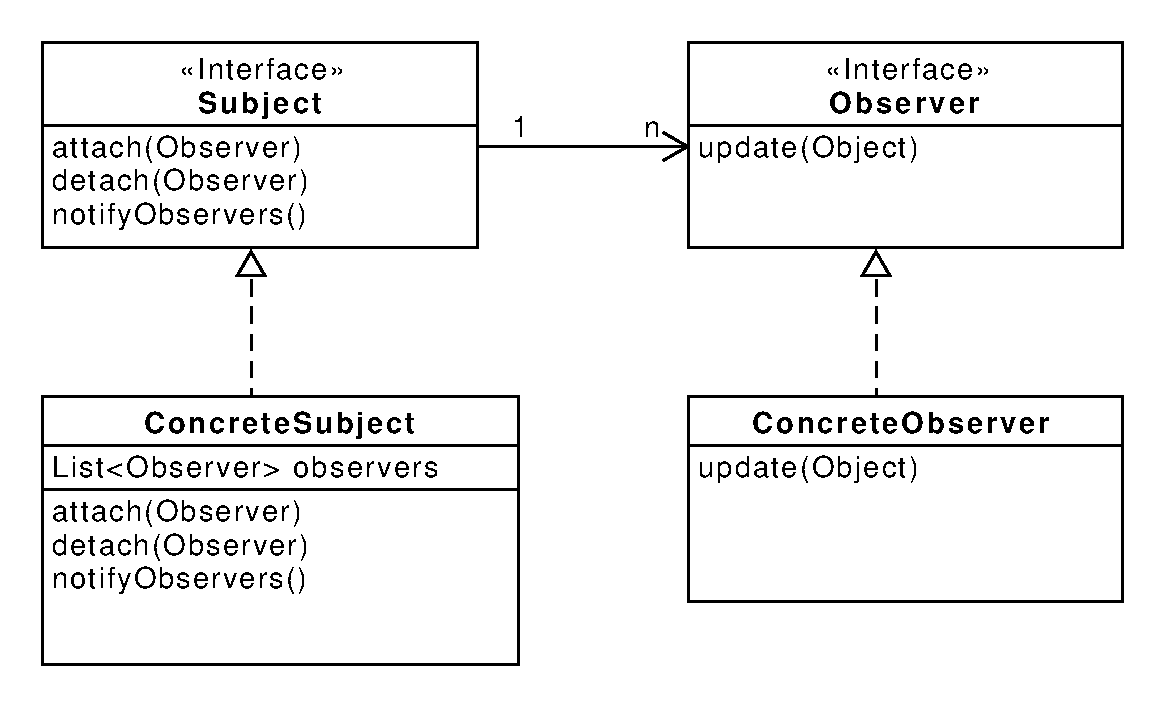
\includegraphics[scale=.37]{paper/observer/observer}
				\end{figure}
  	\end{columns} 
\end{frame}

\subsection{Beispiel - Jobcenter}
\begin{frame}
	\frametitle{Beispiel}
	\begin{itemize}
		\item 1-zu-n-Kommunikation zwischen Jobcenter und Client 
		\item Jobcenter kennt weder Anzahl noch konkrete Clients
		\item Clients bearbeiten ihre Benachrichtigung unterschiedlich
	\end{itemize}		 
  	\begin{figure}
		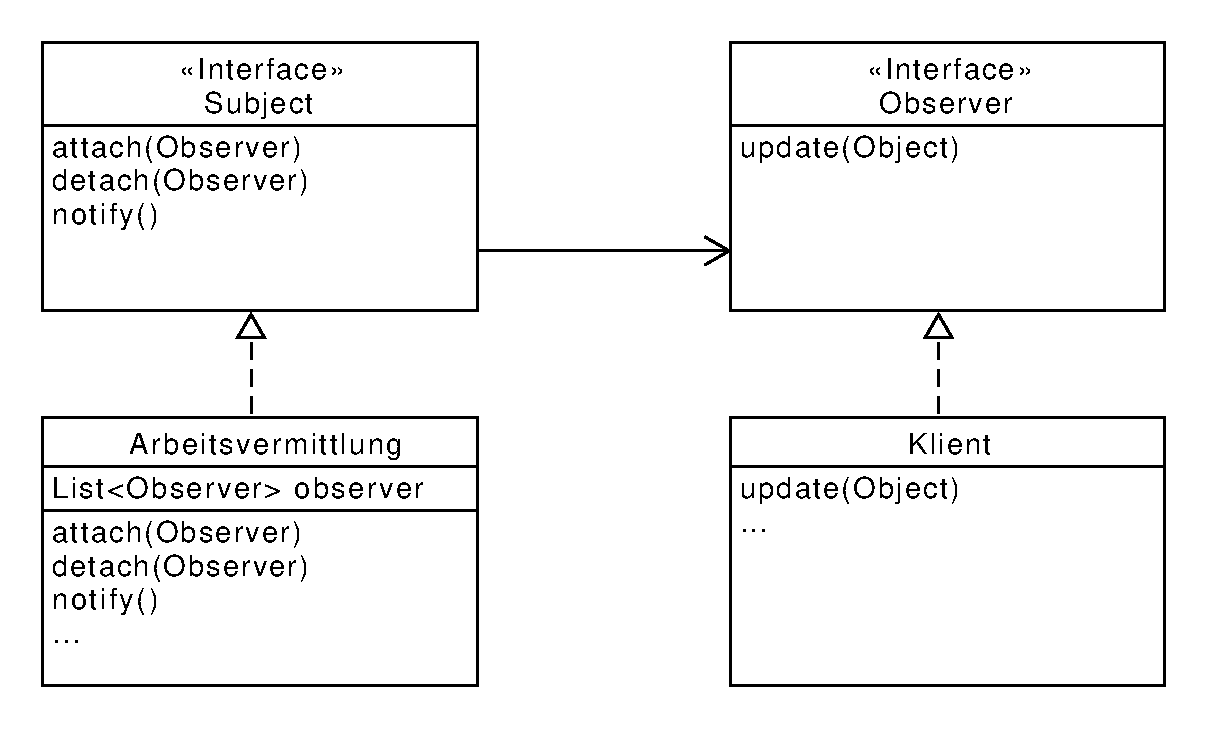
\includegraphics[scale=.4]{paper/observer/arbeitsvermittlung}
	\end{figure}
\end{frame}


\begin{frame}
\frametitle{Beispiel}

		\javacode{resources/observer_Subject_Interface.java} 
		\javacode{resources/observer_Arbeitsvermittlung.java}	  
\end{frame}

\begin{frame}
\frametitle{Beispiel}
		\javacode{resources/observer_Observer_Interface.java}
  		\javacode{resources/observer_Klient.java}	 
\end{frame}

\subsection{Implementierungsmöglichkeiten}
\begin{frame}
\frametitle{Implementierungsmöglichkeiten}
		\begin{block}{Push Modell}
		  \begin{itemize}
		  	\item Subject übergibt detaillierte Informationen 
		  	\item Observer hat keinen Zugriff auf Subject
		  	\item Subjekt muss Interesse der Observer kennen
		  \end{itemize}
  		\end{block}
  		\begin{block}{Pull Modell}
  		 \begin{itemize}
		  	\item Subject informiert nur auf Veränderung und übergibt keine Daten
		  	\item Observer muss sich Daten vom Subject holen
		  	\item Observer müssen Subject kennen
		  \end{itemize}  
  		\end{block}
  		Beides kann auch gemischt werden!
\end{frame}

\begin{frame}
\frametitle{Implementierungsmöglichkeiten}
		\begin{block}{Ausführung der Benachrichtigungsmethode durch Subject}
  		 \begin{itemize}
  		 	\item z.B. in Add-Methoden
		  	\item Weniger fehleranfällig
		  	\item Jedoch zu häufige Updates
		  \end{itemize}  
  		\end{block}		
  		\begin{block}{Ausführung der Benachrichtigungsmethode von Extern}
		  \begin{itemize}
		  	\item Fehleranfälliger
		  	\item Regulierung der Updates
		  \end{itemize}
  		\end{block}	
\end{frame}

\begin{frame}
\frametitle{Implementierungsmöglichkeiten}
		  \begin{block}{Observer beobachten mehrere Subjects}
		  	\begin{itemize}
		  		\item Observer registriert sich bei mehreren Subjects
		  		\item Muss allerdings unterschiedlich darauf reagieren
		  		\item Lösung: Erweiterung der update-Methode mit Subject
		  	\end{itemize}
		  \end{block}
		\javacode{resources/observer_erweiterung_update.java}  		
\end{frame}

\begin{frame}
\frametitle{Implementierungsmöglichkeiten}
		\begin{block}{Observer gibt sein Interesse an}
  		 \begin{itemize}
		  	\item Observer registrieren sich für ein bestimmtes Event
		  	\item Subject kümmert sich um die Zuordnung
		  	\item Benachrichtigung wird effizienter
		  	\item Subject wird komplexer
		  \end{itemize}  
  		\end{block}		
  		\javacode{resources/observer_sortToObserverlist.java}  
\end{frame}

\begin{frame}
\frametitle{Implementierungsmöglichkeiten}
		\begin{block}{Einführung eines \texttt{ChangeManager}}
  		 \begin{itemize}
		  	\item Subject delegiert Aufgaben zu ChangeManager
		  	\item ChangeManger hat drei Aufgaben:
		  	\begin{itemize}
		  		\item Legt Zuordnung von Subject, Observer und Demand fest
		  		\item Legt Aktualisierungsstrategie fest
		  		\item Führt die Aktualisierung aus
		  	\end{itemize}
		  \end{itemize}  
  		\end{block}		
  		\begin{figure}
		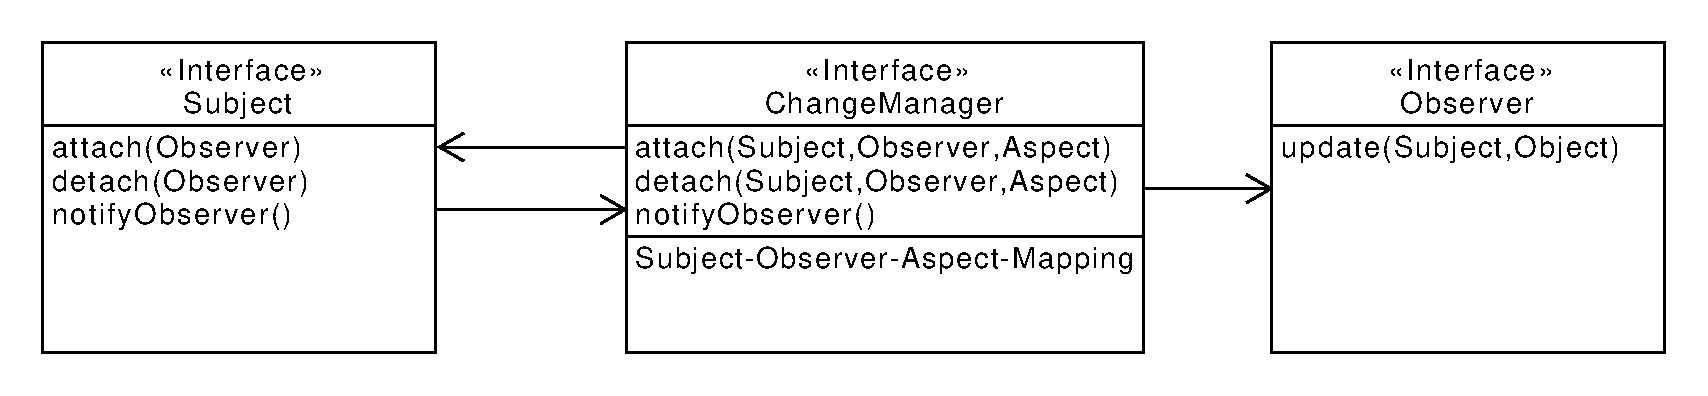
\includegraphics[scale=.4]{paper/observer/changemanager}
	\end{figure}
\end{frame}

%\begin{frame}
%\frametitle{Observer-Pattern als Fehlerquelle}
%		\begin{block}{Konsistenz vor dem Update}
%			\begin{itemize}
%  				\item Vorsicht bei Vererbung
%  			\end{itemize}  
%  		\end{block}		
%	\begin{block}{Verwaiste Referenzen auf gelöschte Subjects}
%			\begin{itemize}
%  				\item Subject wird gelöscht und Observer wissen nichts darüber
%  			\end{itemize}  
%  		\end{block}	
%  		\begin{block}{Komplexe Strukturn}
%			\begin{itemize}
%  				\item Zyklische Abhängigkeiten
%  				\item Komplexe Fehlersuche
%  			\end{itemize}  
%  		\end{block}			
%\end{frame}


\subsection{Fazit}
\begin{frame}
	\frametitle{Fazit}
	\begin{columns} 
    	\column[t]{.50\textwidth} 
    		\begin{exampleblock}{Vorteile}
    			\begin{itemize}
    				\item Lose Kopplung
    				\item Flexibilität
    				\item Automatische Benachrichtigung
    			\end{itemize}
    		\end{exampleblock}
    	\column[t]{.50\textwidth} 
    		\begin{alertblock}{Nachteile}
    			\begin{itemize}
    				\item Komplexität
    				\item Gefahr von Zyklen
    			\end{itemize}
    		\end{alertblock}
  	\end{columns}   	  		
\end{frame}